\documentclass{article}
\usepackage[utf8]{inputenc}
\usepackage{graphicx}
\graphicspath{ {./images/} }

\title{\textbf{Lightweight Restaurant Management System} \\CS699 Software Lab Project \\Indian Institute of Technology, Bombay}
\author{\textbf{Team: BugBusters}\\ Sushil Kukreja 203050020\\ Ankit Raj 203050047\\ Sumit Thorat 203050087\\ Ramswaroop None 203050117}
\date{18th November 2020}

\begin{document}

\maketitle

\section{Introduction}
Lightweight Restaurant Management System is a software system which aims to digitise the order management process at restaurants whilst being very light, inexpensive and user friendly. It does so by enabling the restaurant staff to make use of an Android app to view orders, edit menu, manage tables and view statistics. IT allows placing orders using a webapp which can be accessed via a table specific QR code. 

\section{Motivation}
During this time of peril where Covid-19 is causing havoc, we are moving
towards the new normal of masks and social distancing. One such place where there is high amount of exposure to the virus is a
restaurant. Everybody loves to eat outside once in a while but the risks
attached with it are higher than normal. This system would reduce the contact between various people to bare minimal by leveraging the power of technology. Being lightweight and inexpensive, even small scale restaurants can make use of this system to their advantage.

\section{Dependencies}
\begin{itemize}

    \item{Python Django}
    
    \item{Python Flask}
    
    \item{Python Socketio}
    
    \item{Python PyQRcode}
    
    \item{Android Mobile Phone}

\end{itemize}

\section{Usage}
Get the system up and running by executing the following commands when in the project directory.

\begin{itemize}
    \item{pip3 install -r Backend/API/requirements.txt}
    
    \item{python3 Backend/API/main.py}
    
    \item{python3 Backend/Webapp/PROJECT/manage.py runserver}
    
    \item{Install the APK Frontend/Android/app-debug.apk in the Android phone}
\end{itemize}

\newpage
\subsection{Android App}
Users need to register themselves before accessing the app. After registering for the first time, users can login using the login page.
\begin{center}
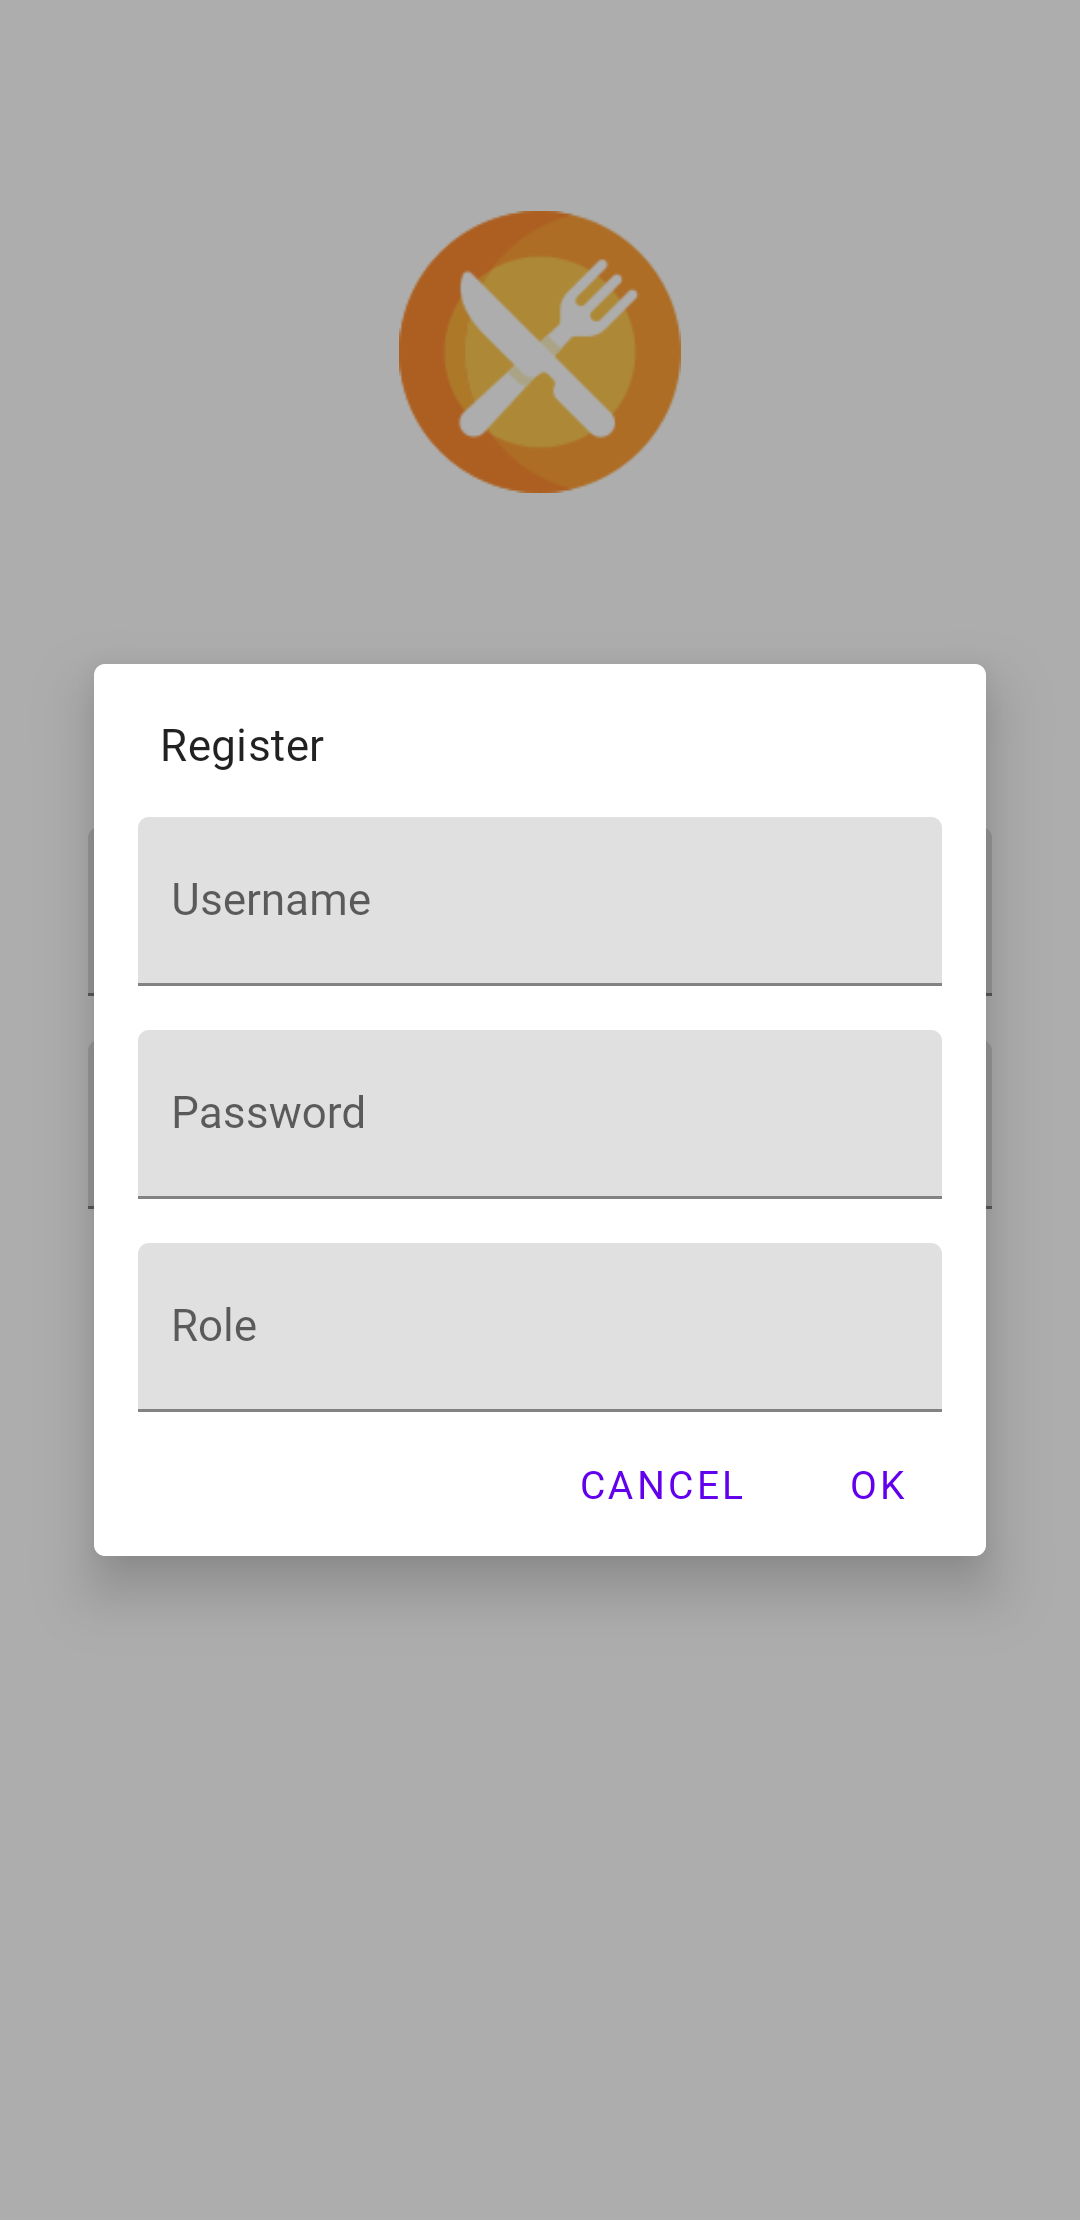
\includegraphics[scale=0.15]{register}
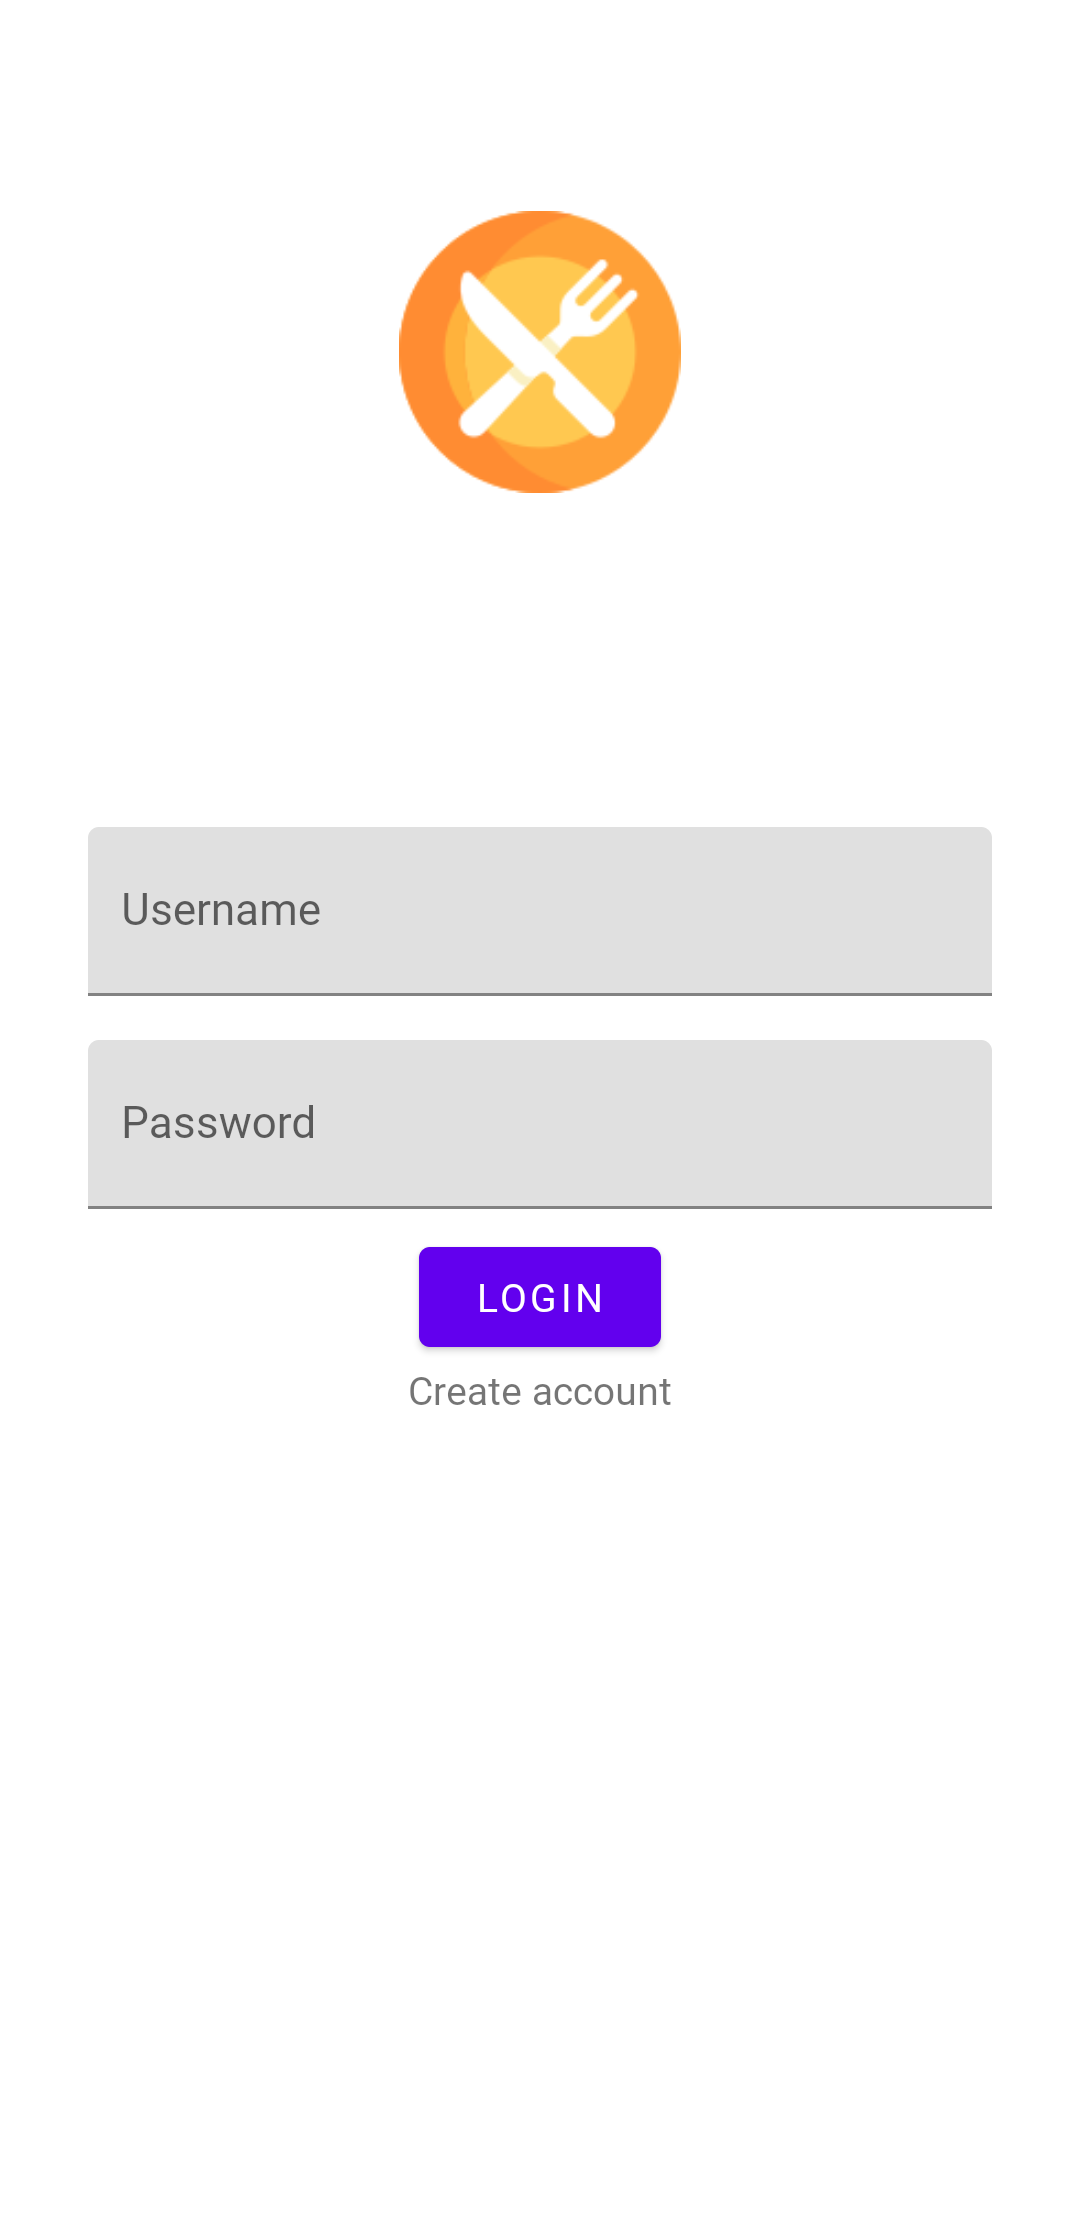
\includegraphics[scale=0.15]{login}
\end{center}

\newpage
Pending orders can be seen on the View Orders page. Orders here can be marked completed by swiping on the card from right to left.
\begin{center}
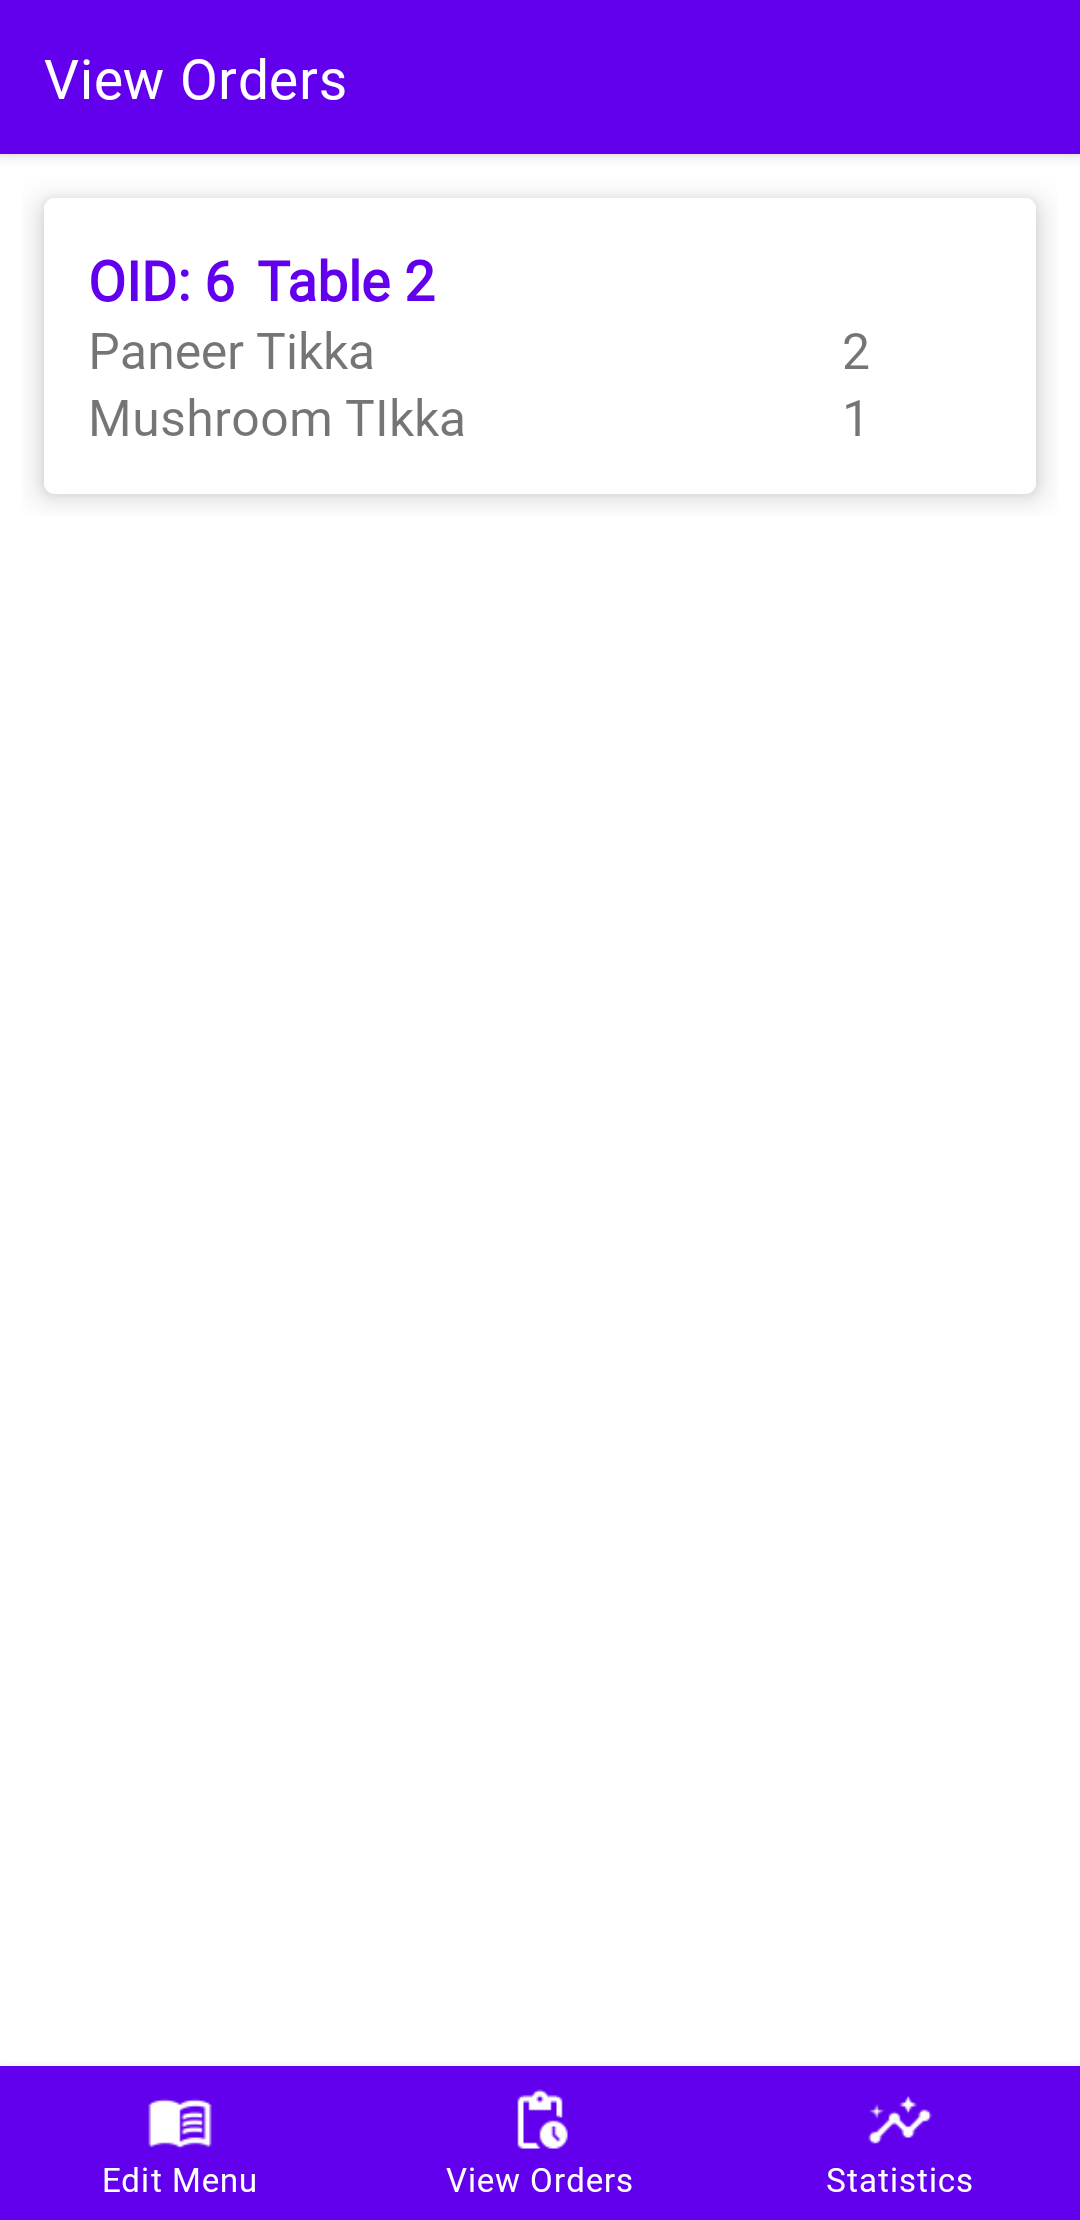
\includegraphics[scale=0.15]{view-orders}
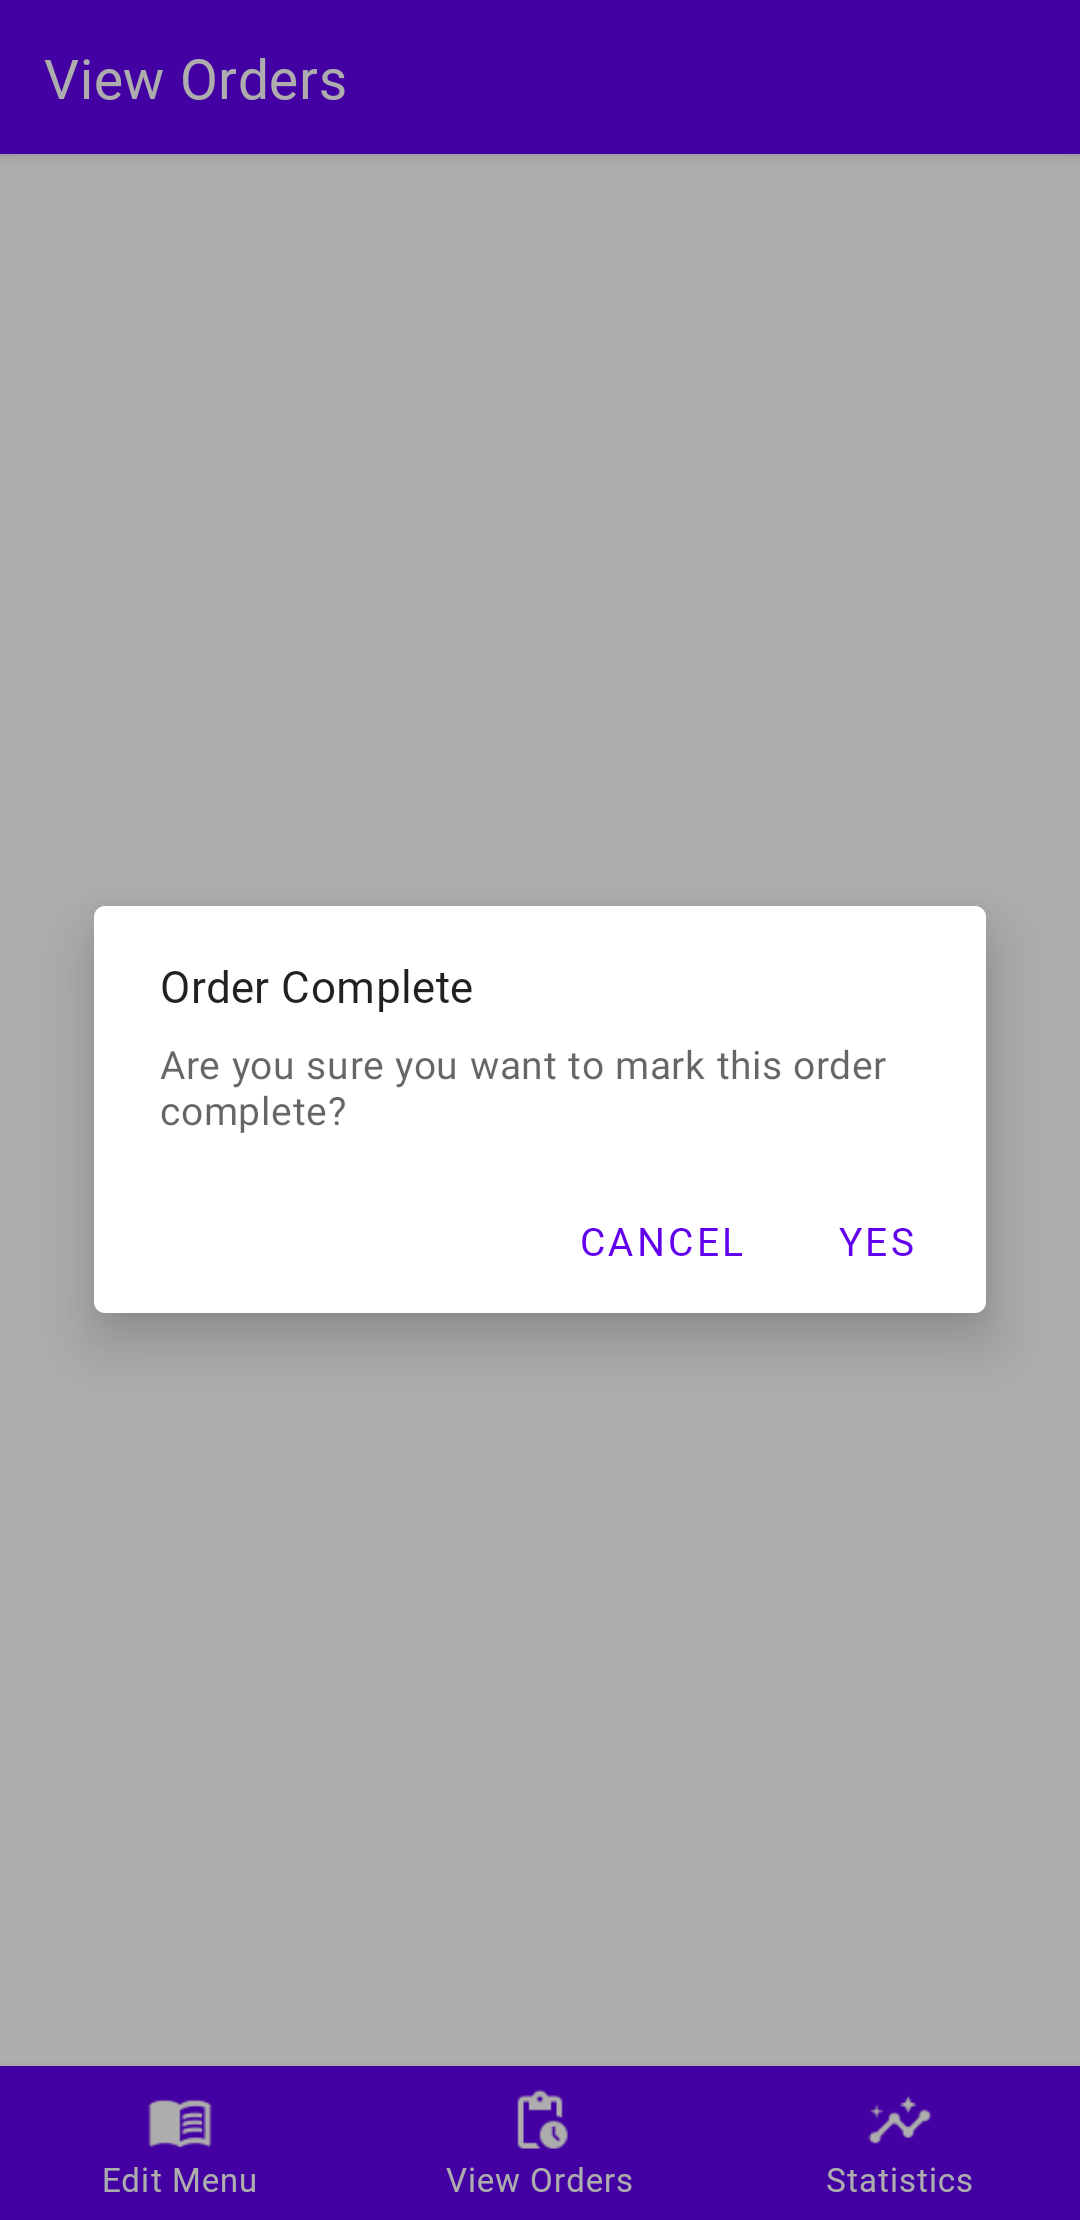
\includegraphics[scale=0.15]{complete-order}
\end{center}

\newpage
Current menu can be viewed on the Edit Menu page. New menu items can be added by tapping on the Add Item button. Users can add a new category or select from a pre-existing category.
\begin{center}
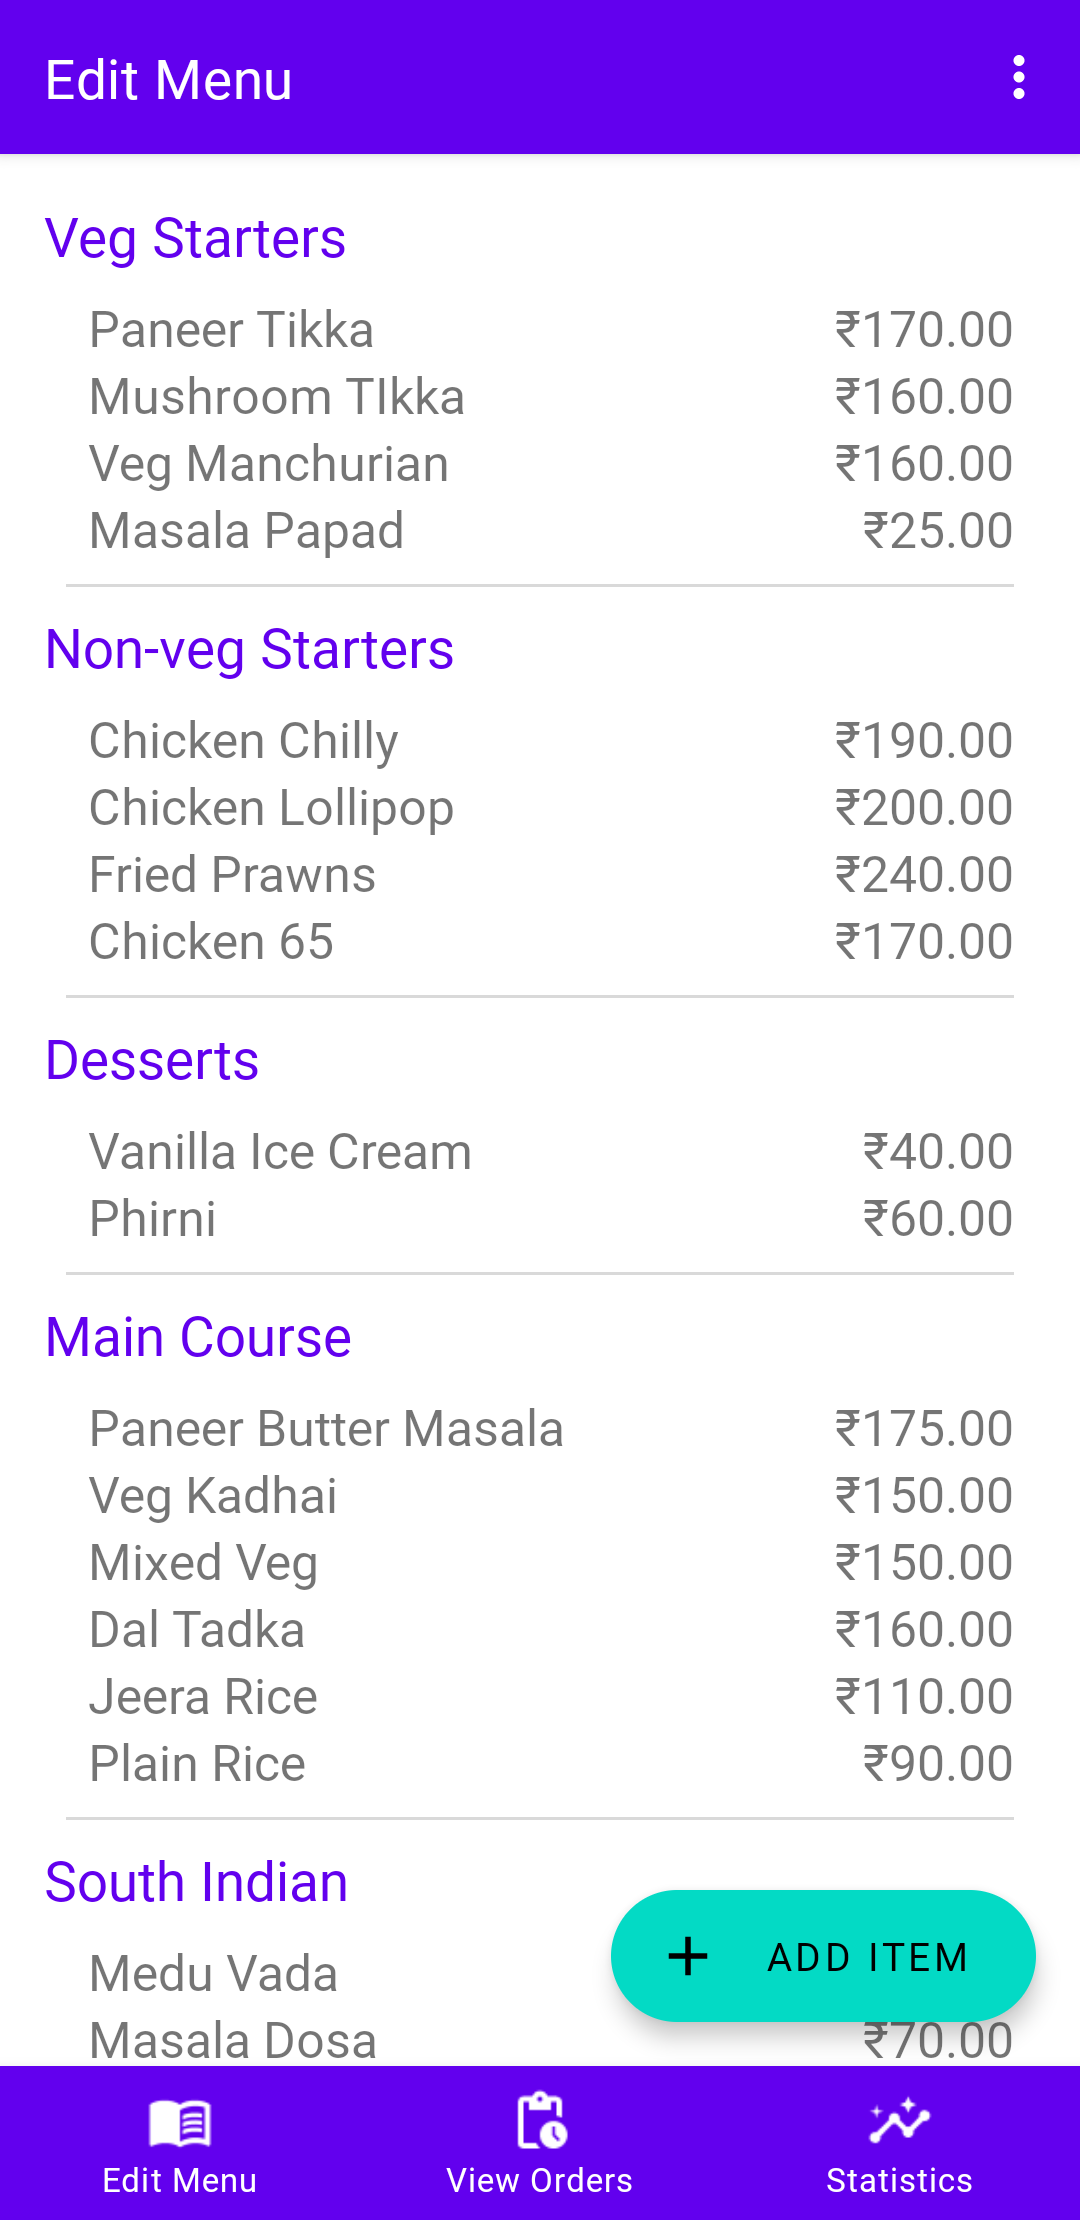
\includegraphics[scale=0.15]{view-menu}
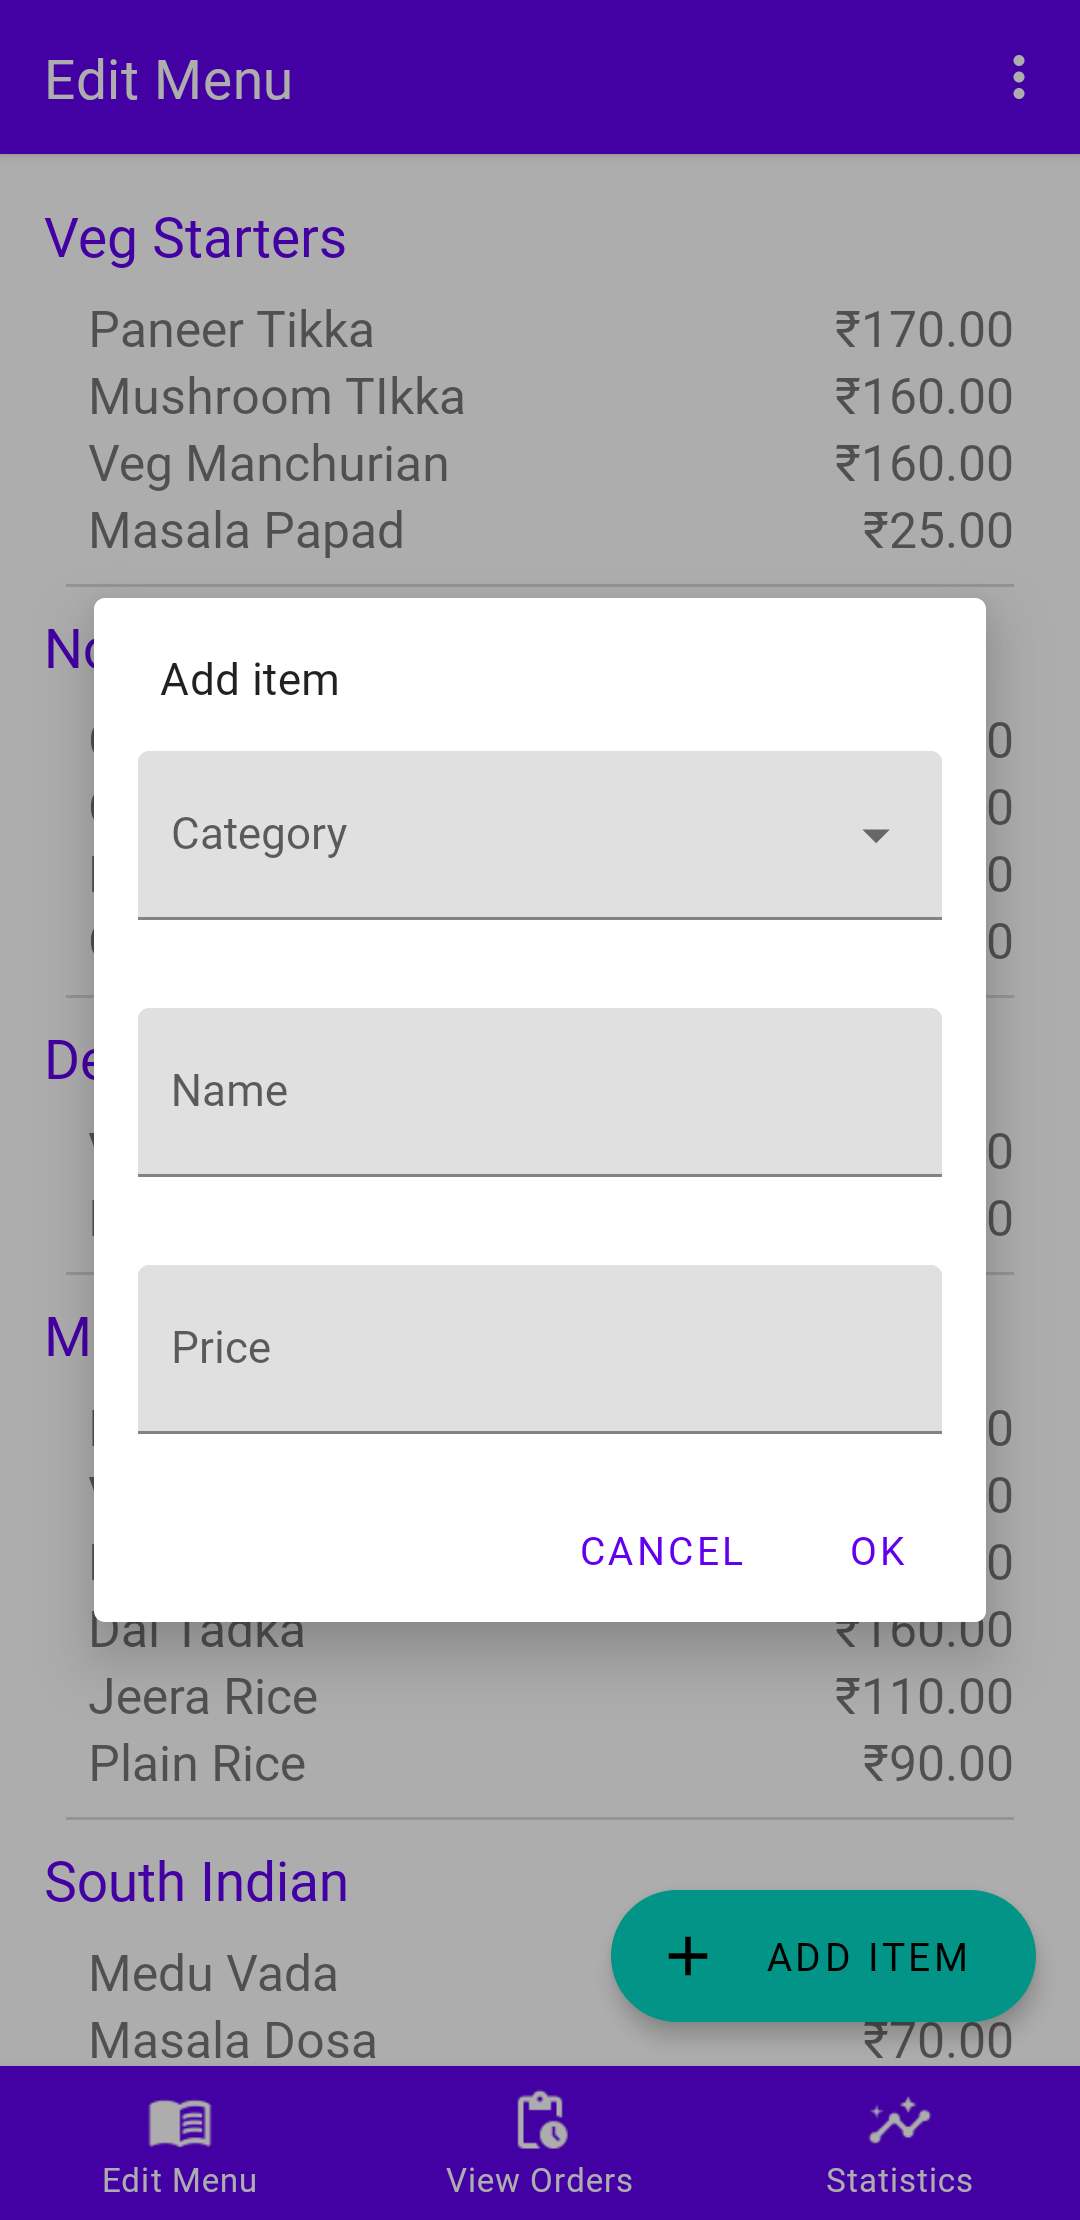
\includegraphics[scale=0.15]{add-item}
\end{center}

\newpage
Tables can be managed by clicking on the options icon in the Edit Menu page and selecting Manage Tables. Here, users can share the QR code for each table to print it or delete the table by clicking on the delete icon. New tables can be added by tapping the add icon in the top right corner of the Manage Tables page. \begin{center}
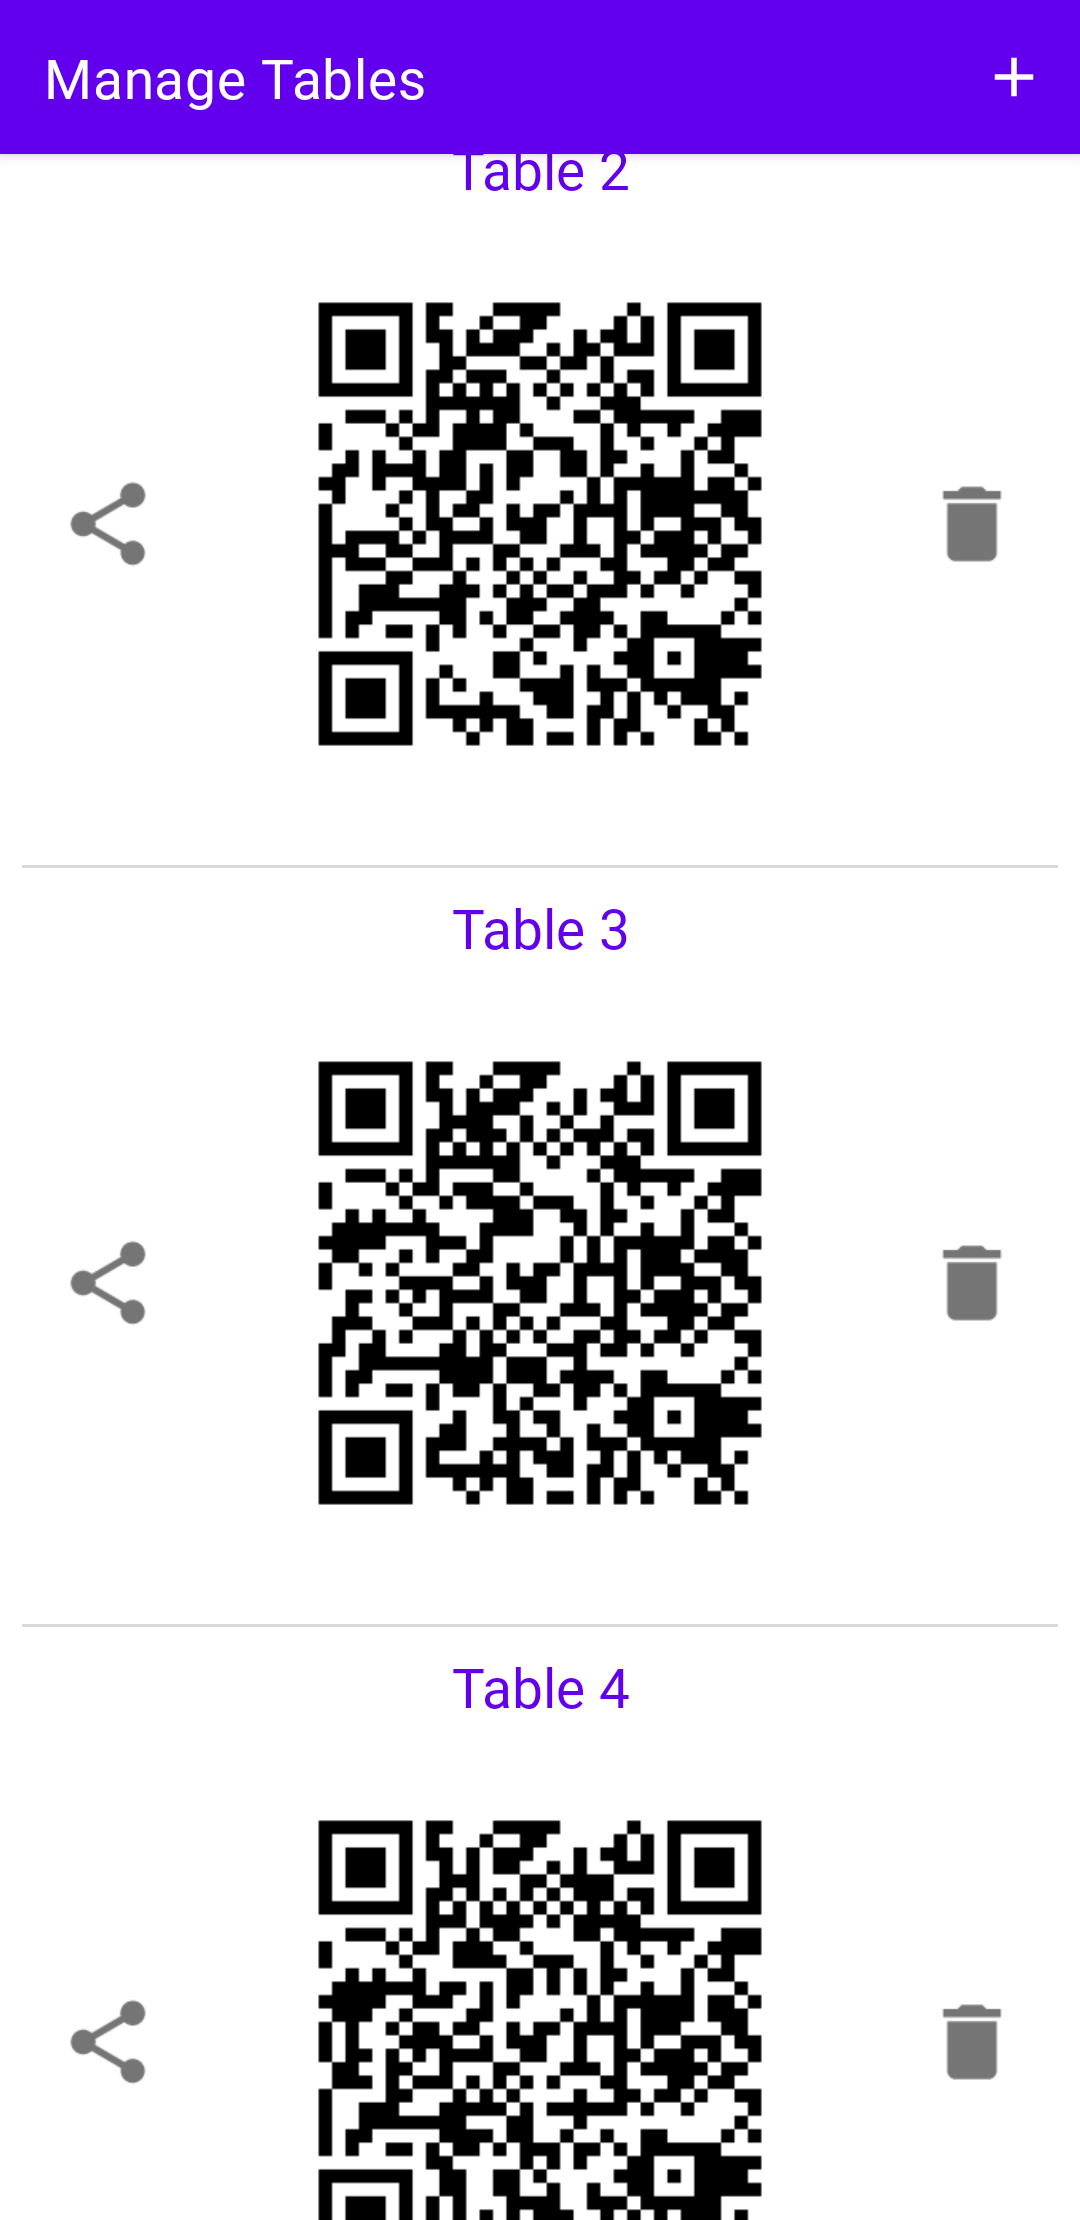
\includegraphics[scale=0.15]{manage-tables}
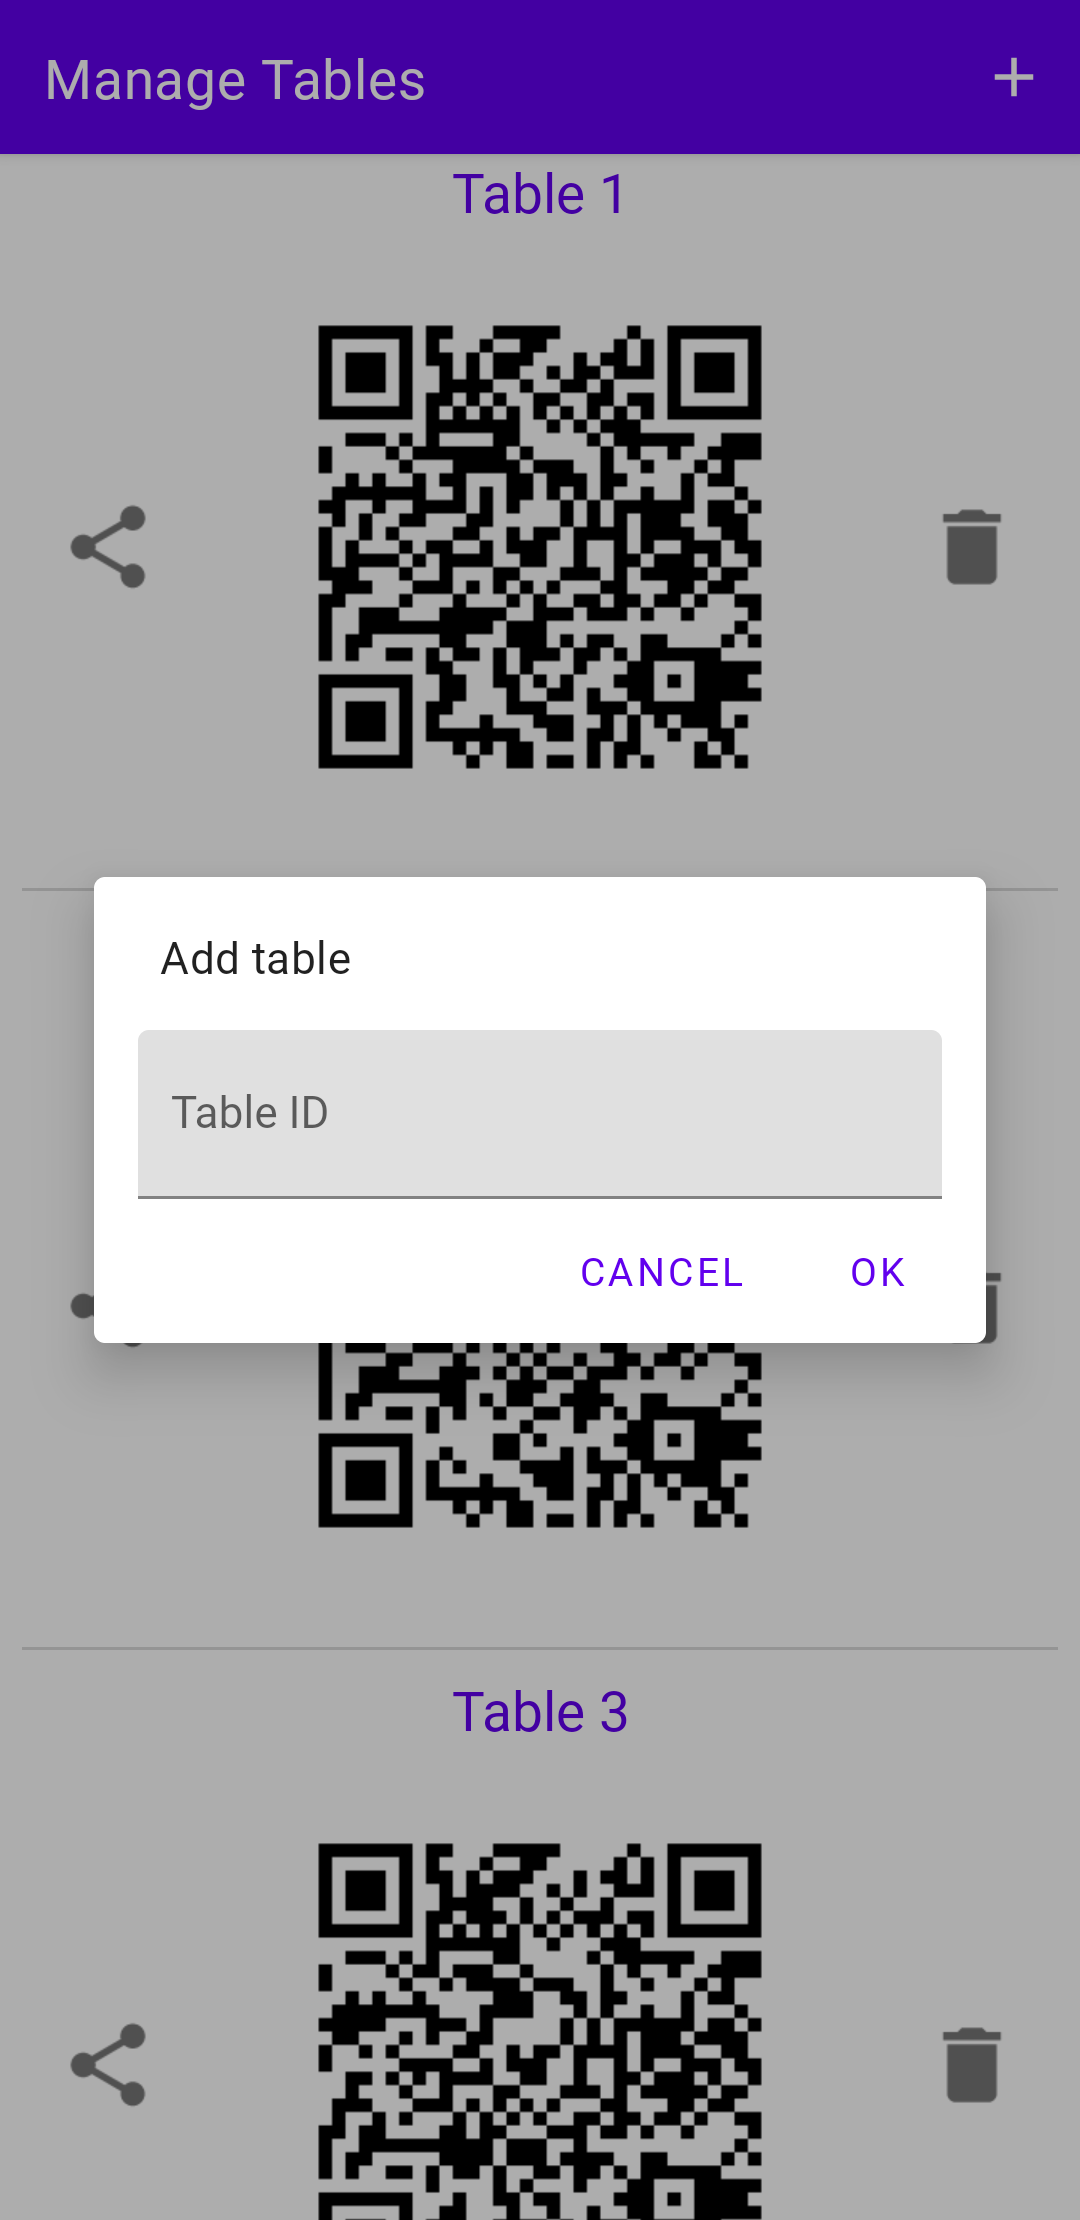
\includegraphics[scale=0.15]{add-table}
\end{center}

\newpage
Statistics such as average order completion time, most sold item of the day, total item sale for a given item can be viewed on the Statistics page. Users can enter the item name for which the item sale so far is required and tap on the get button to get the quantity. 

\begin{center}
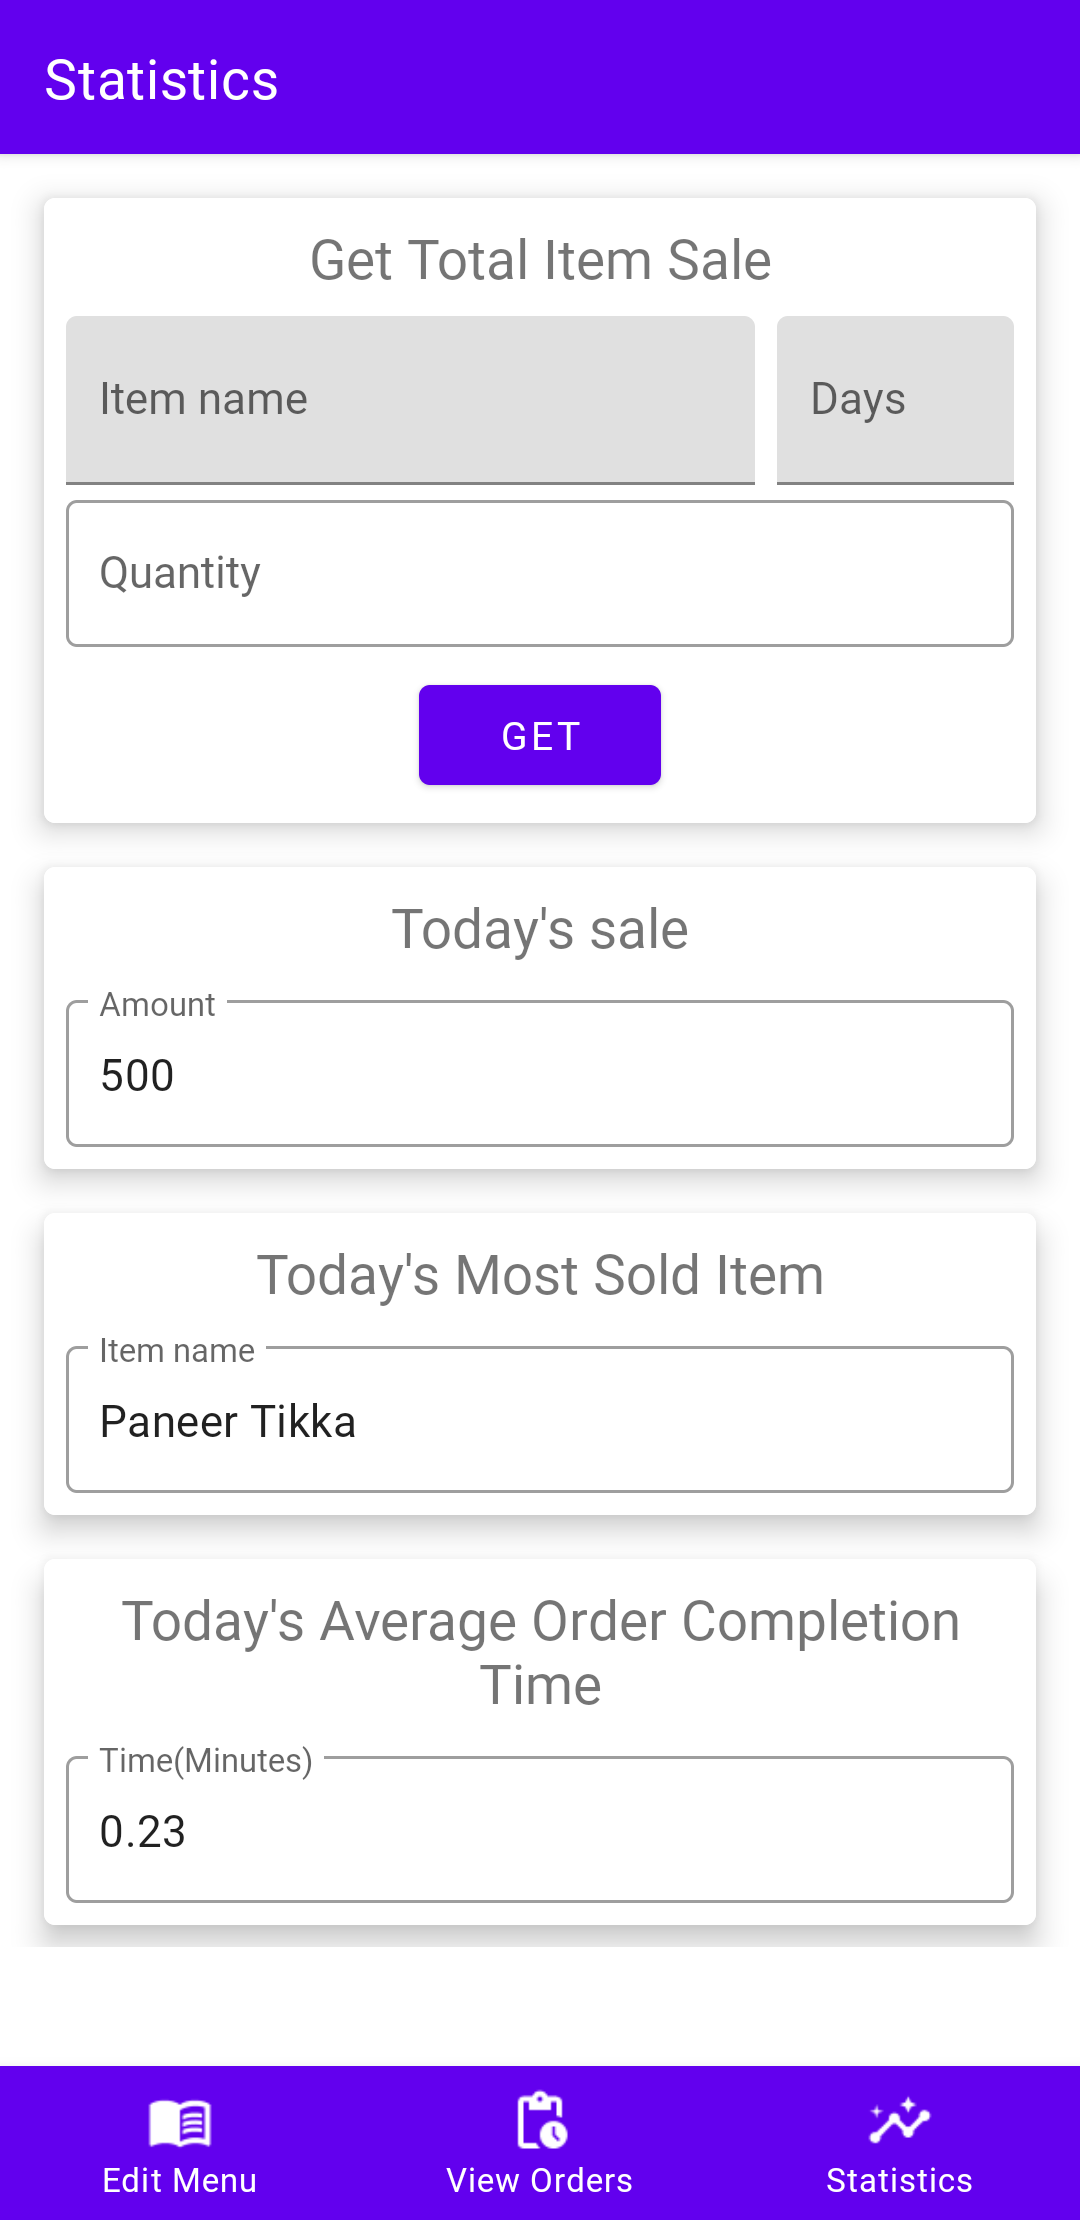
\includegraphics[scale=0.15]{statistics}
\end{center}

\newpage
\subsection{Webapp}
After scanning the table specific QR code, users will be redirected to a webpage which will allow placing orders. Users need to select the corresponding item's checkbox and enter the quantity then click on the Place Order button. An alert will be shown when the order is placed.
\begin{center}
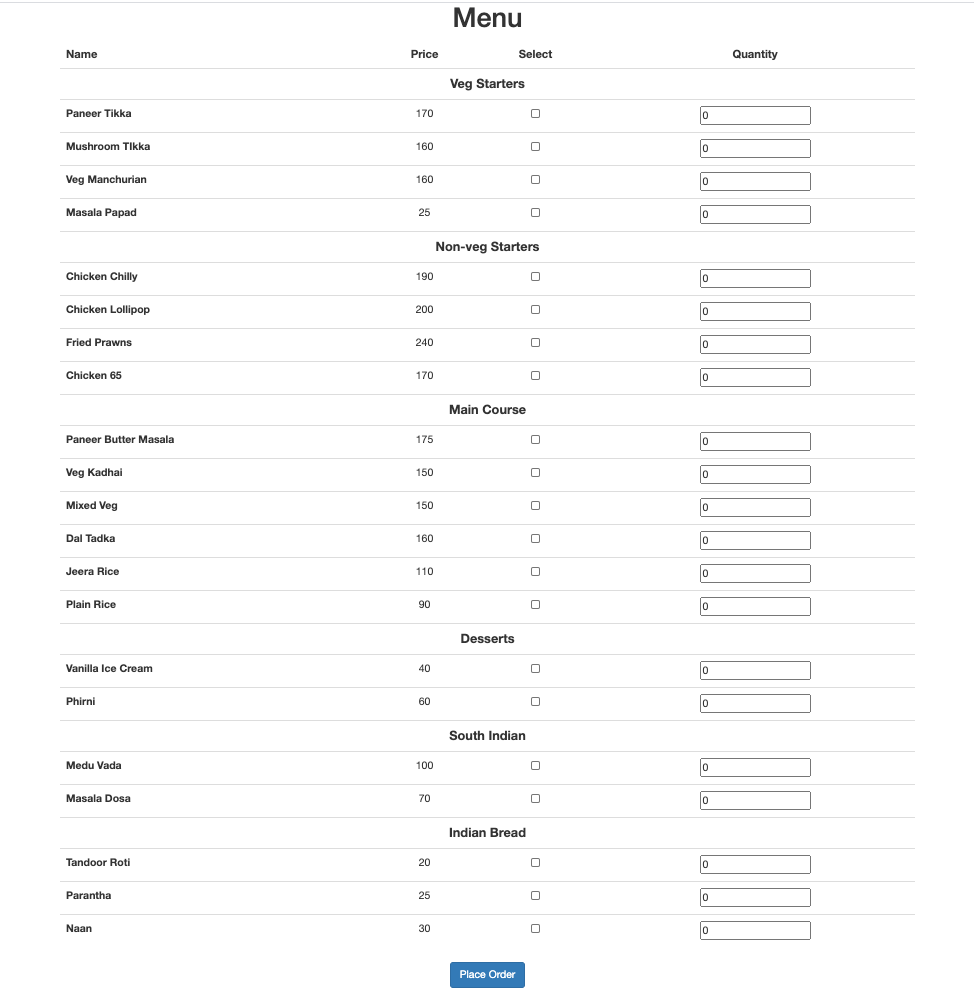
\includegraphics[scale=0.4]{webapp}
\end{center}

\newpage
\section{Future Scope}
\begin{itemize}
    \item{A digital token system can be implemented which will allow placing orders only after a token has been given to the customer.}
    
    \item{The base webpage can be used to showcase the brand page of the restaurant.}
    
    \item{Support for iOS. }

\end{itemize}
    

\end{document}
